\chapter{Introduction}\label{cha:intro}

\section{Background}
The ratio between Heterophils and Lymphocytes in chickens is a useful measure of their stress level \cite{hlratio}. As of now this ratio is calculated by hand, by using a digital slide scanner and counting the cells in the resulting image. This is a very laborious and time consuming task. This thesis analyses the possibility of automating this process, completely or partially, in conjunction with an interactive graphical user interface for manual correction.\\\\
The goal is that it will be a usable application for researchers in biology and similar fields, without degrees in engineering or other strictly technical fields.

\section{Biological background}
\subsection{Red blood cells}
The red blood cells in avian species have a cell nucleus, which mammalian red blood cells do not. This makes it harder to distinguish them from the white blood cells, which is one of the main reasons that cell recognition software for humans and other mammals cannot directly be applied to avian blood smear images.
\subsection{White blood cells}
White blood cells, or leukocytes, are cells of the immune system that are involved in protecting the body against infectious diseases, e.g. from viruses, bacteria or parasites. Both Lymphocytes and Heterophils are white blood cells.
\subsubsection{Heterophils}
Heterophils are a type of granulocyte that occurs in most avian species. Granulocytes are a category of leukocytes characterized by the presence of granules in their cytoplasm, that are more or less visible in the blood smear images. Heterophils in avian species are functionally equivalent to neutrophils in most mammal species.

\begin{figure}[h!]
    \centering
    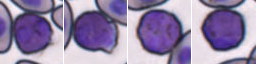
\includegraphics{heterophils_.png}
    \caption{Heterophils from a 9 week old chicken.}
    \label{fig:heterophil}
\end{figure}

\subsubsection{Lymphocytes}
Lymphocytes are smaller leukocytes with a large nucleus. They are sometimes confused with platelets, which are often smaller and darker than the lymphocytes. Platelets are also commonly referred to as thrombocytes and their function is to stop bleeding and clotting injured blood vessels \cite{NYAS:NYAS297}.
\begin{figure}[h!]
    \centering
    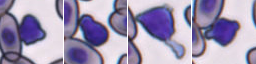
\includegraphics{lymphocytes_.png}
    \caption{Lymphocytes from a 9 week old chicken.}
    \label{fig:heterophil}
\end{figure}

\section{Problem description}

\begin{center}
  \makebox[\textwidth]{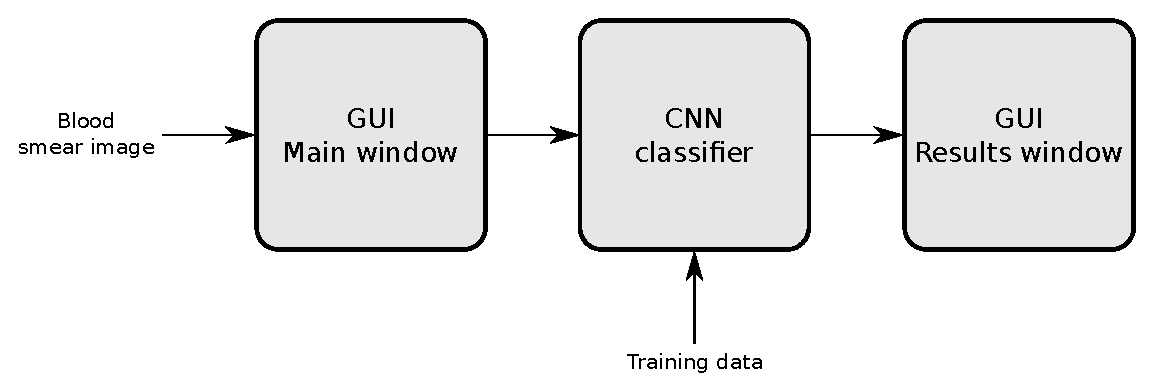
\includegraphics[width=\textwidth]{exjobb_bild.eps}}
\end{center}
Color images of blood cells from peripheral blood smears are taken with a digital microscope, and different types of blood cells are to be segmented and classified using a convolutional neural network (CNN). The most important blood cells are heterophils and lymphocytes, other white blood cells such as monocytes, eosinophils and basophils are not important for the task at hand, but it can be beneficial to detect these as well.\\\\
The images are given in the ndpi format, which is basically a proprietary extension of the TIFF file format, with different zoom levels of the blood smears. This application will only use the ones that are taken with the largest zoom available, in which a white blood cell occupies an area of approximately 50x50 pixels.\\\\
From the images a ground truth must be established. This is done by manually cropping out the individual cells and saving them as PNG images, with a number in the name corresponding to its class. Since the cells are seldom isolated in the image, it is expected that almost all individual cell images will contain parts of other cells around it. 
Since the CNN algorithm is much like a black box in terms of insight into the network from the user's perspective, thorough testing must be done with the trained network so as to verify the accuracy and flexibility.

\section{Calculation of accuracy}
The accuracy is calculated as precision, recall and F score. More on this in the Results chapter.

\section{Limitations}
There are several limitations to this thesis, the main ones will be mentioned here.

\subsection{Data set}
There are hundreds of images available, where each image is in the order of $10^{10}$ pixels. However, since labelling is time consuming only a few thousand white blood cells have been labelled in these images. In this thesis, around 10-20 of the available images have been used. The data set only contain blood smear images from chickens of the age of 9 and 12 weeks, which probably limits the robustness of the application, since the cells vary in size and shape during the chickens lifetimes.\\
The color and quality of the blood smear images can vary when scanning and/or staining them, so to keep the algorithm as unbiased as possible to specific images, the cut out learning images are taken in equal amounts from the selected part of the available images.

\subsection{Loss of depth}
When manually analysing a blood smear image in a microscope, it is possible to set the focus to different depths of a cell. This can make it easier to correctly classify the type of the cell, since some features are more apparent at other depths. Since the cells are essentially photographed at a fixed depth, any other information about the cell that could be found on another focus plane will be lost.
However, since the modern method of counting the cells by hand most often use the same digital blood smear images as those that are used in this thesis, and seldom involves manually counting the cells through a microscope, the loss of depth is thus not limited to our method.

\subsection{Image artefacts}
Getting a perfect image from a blood smear image is virtually impossible. The concentration of blood cells in the image varies significantly, in some parts the cells may be clumped together in groups of several hundred cells, in other parts the cells are spread very far apart. There are also many damaged cells from the smearing process, and strands of hair and dust is quite common. When analysing the images manually, the most common method is to choose a few regions of interest ( ROI) where the amount of artefacts is low, and the concentration of cells is at an acceptable level.\\\\
The approach used in this thesis has been to automatically cut a blood smear image into squares with a size of 2048 by 2048 pixels, saving them as TIFF images, sorting them by size in kilobytes, which crudely sorts them after cell density, since images with few cells will be more efficiently compressed. Finally, a few ROIs were chosen manually from somewhere in the middle of this list, where the cell density was not too high or too low, and the amount of artefacts are minimal.

\subsection{Ambiguity in classes}
The different types of blood cells can sometimes look very similar to each other, making it difficult even for trained humans to accurately classify these cells\cite{Bohls2006843}. This owes to individual differences in the chickens. The size and color of the cells can vary greatly even in the same blood smear image. There are always a number of cells that got damaged in various degrees when producing the blood smear images, which makes the classification even harder. These cells are often not taken into account when counting them manually though.\\\\
This has been the hardest problem to solve in this thesis, and remains somewhat unsolved. The lymphocyte cells especially can be very similar to partially broken red blood cells, and a trade-off had to be done between either often missing some lymphocytes while not falsely classifying red blood cells as lymphocytes, or less often missing lymphocytes while falsely classifying red blood cells as lymphocytes. The resulting algorithm leans more towards falsely classifying damaged red blood cells as lymphocytes, as it is more important not to miss lymphocytes. This has been achieved by removing some of the damaged red blood cells from the training images, so that the classifier is not as strict when it comes to classifying them.

\subsection{Calculation of accuracy}
The previously mentioned limitations and issues makes the calculation of the accuracy hard to determine. Therefore, some choices had to be made regarding issues in determining cell types. If the classifier fails to mark a heterophil or lymphocyte that could be seen as damaged, but is present in the ground truth image, it is not taken into account when determining the precision. If it marks a heterophil or lymphocyte that could be seen as damaged, but is not present in the ground truth image, it is not taken into account when determining the recall. Examples of these are given in the Results chapter.

\subsection{Human blood smear comparison}
The problem of counting leukocytes in human blood smears is largely solved\cite{5190593}\cite{hiremath2010automated}, but for avian species the problem is significantly more challenging to solve, mainly because their red blood cells have nuclei, which the human counterpart does not. A comparison of human and avian blood smear images can be seen in Figure \ref{fig:comparison}. It is readily apparent in this image that the human blood smear images are easier to automatically classify, since the blood cells in the human image have simpler shapes and textures. Figure \ref{fig:sneaky} shows comparisons between lymphocytes and especially hard to classify red blood cells.

\begin{figure}[h!]
    \centering
    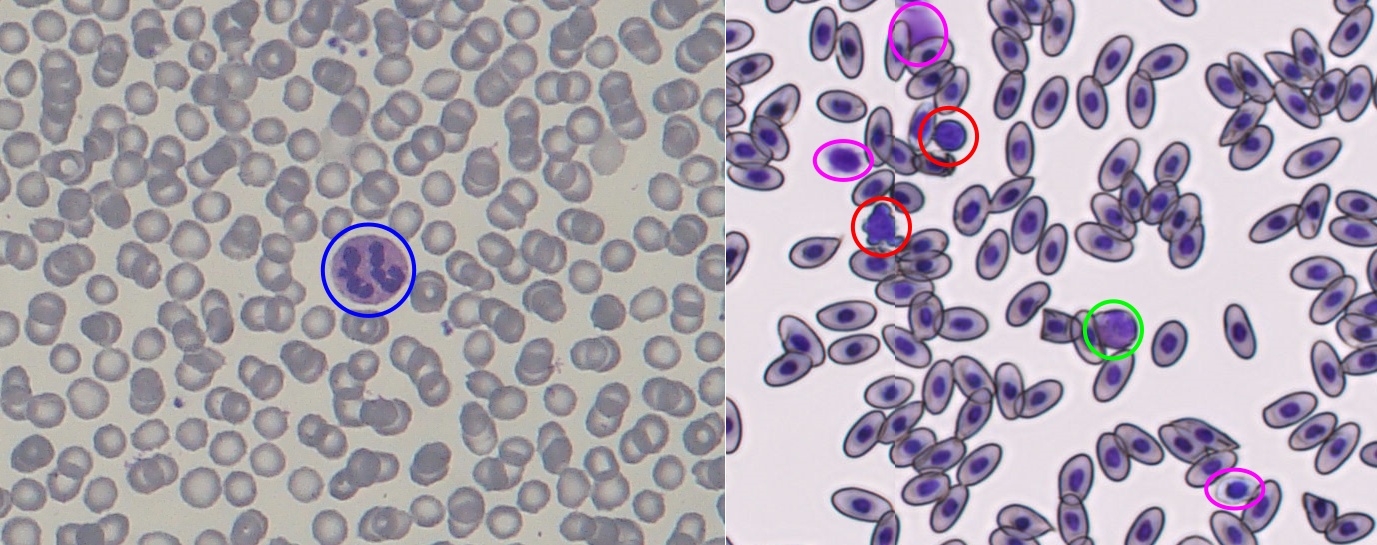
\includegraphics[width=\textwidth]{comparison_marked_}
    \caption{Comparison of human (to the left) and avian (to the right) blood smears. The unmarked cells in both images are red blood cells. The blue in the left image is a neutrophil, the red, green and pink in the right are lymphocytes,  heterophils, and various damaged red blood cells respectively.}
    \label{fig:comparison}
\end{figure}

\begin{figure}[h!]
    \centering
    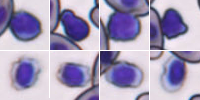
\includegraphics[width=\textwidth/2]{comparison_sneaky_}
    \caption{The top four images show lymphocytes, and the bottom four undecided or broken red blood cells. These are hard even for an expert to correctly classify.}
    \label{fig:sneaky}
\end{figure}
